\section{Characterization Problem Results}
\label{sec:CharResults}

To quantify the $\Omega$-method success for a variety of anisotropy-inducing
physics, we will present various forms of the Figure of Merit, as described in
Section \ref{sec:successmetrics}.
In the preceding subsections, a
subset of flux anisotropy-inducing physics have been identified
and a subset of problems that contain these physics have been conceived.
In this section, the results for CADIS-$\Omega$, CADIS, and nonbiased Monte Carlo
will be presented for each of these problems. Explanations on the performance of
the $\Omega$ methods will accompany the results for each problem. In some cases,
variants of problems were run to confirm or refute observations seen
in other problems.

\subsection{Computational Specifications}
\label{subsec:comp_specs}

As noted in a number of the previous sections, hybrid methods require both a
deterministic and a Monte Carlo calculation to obtain a problem result. These
transport codes require different computational parameters to obtain an answer.
For the characterization problems the computational parameters are summarized in
Table \ref{tab:simulation_defaults}; the parameters for the deterministic and
Monte Carlo calculations are demarcated in the table.

\begin{table}[h!]
  \centering
  \begin{tabular}{l|m{5cm}}
\toprule
Parameter Type & Parameter Value \\
\midrule \midrule
\multicolumn{2}{c}{ADVANTG Values$^1$} \\
\midrule
P$_N$ Order               &    $3$ \\
Quadrature Type           &  Quadruple Range \\
Quadrature Order          &    $10$ \\
Spatial Solver            &  Step Characteristic \\
Energy Group Library$^{\dagger}$     &    27G19N \\
Boundary Conditions & vacuum \\
\midrule \midrule
\multicolumn{2}{c}{MCNP Values$^2$} \\
\midrule
Particle Count      &   $1e7$ \\
Boundary Conditions & vacuum \\
\bottomrule
\end{tabular}
\begin{flushleft}
\footnotesize{
  $^1$ ADVANTG runs of the characterization problems
  were run on 16 cores of a 32 core node, with 256Gb of memory on
  an Oak Ridge National Laboratory compute cluster maintained by the Radiation
  Transport and Nuclear Systems Division. \\
  $^2$ MCNP runs of the characterization problems were run on the same
 machine, with 256Gb of memory but using all 32 cores of the node. \\
  $^{\dagger}$ Parameter type that has no default in ADVANTG.}
\end{flushleft}


  \caption[Default simulation values for characterization problems.]{
    Default simulation values for the characterization problems. The values for
    ADVANTG primarily signify parameters used to run Denovo, with exceptions for
    calculating biasing parameters, which is done exclusively in ADVANTG.
    MCNP-specific values are those used for Monte Carlo runs.
  }
  \label{tab:simulation_defaults}
\end{table}

The first portion of the table summarizes the values used by ADVANTG. Note that
these values all pertain to the Denovo deterministic solver, which is set up by
ADVANTG. The parameter types marked with an asterisk have no default in ADVANTG.
We have chosen to use a relatively course 27 group energy group library.
Because the characterization problems are meant to identify the method's
performance pertaining to flux anisotropy, and we expect the energy group
structure to have little effect on anisotropy conditions, we opted for a
computationally inexpensive energy group mesh for the deterministic solver.
The values without an asterisk are ADVANTG default values.
They are also good choices for
initial characterization of the method. This is because a novice user may opt to
use these parameters for an initial solution on a problem for which they may have
little intuition. Further, these values are defaults in ADVANTG for their
computational stability--such as not having negative valued weights or fluxes,
stable convergence, a relatively fast time to a solution, etc.--so they should
be good initial parameters with which to study the characterization problems.

The latter section of the table summarizes the Monte Carlo code MCNP values for
each of the problems. The value of $1e7$ particles as a particle cutoff
was chosen because it made the
error bins in the majority of the nonbiased Monte Carlo
characterization problems less than 100\%. In some problems that are
extraordinarily difficult for Monte Carlo to solve without biasing, there were
tally bins with very high errors. In the following subsections they will be
clearly indicated and their results will not be plotted so as to not obfuscate
the CADIS and CADIS-$\Omega$ results. Time cutoffs were not chosen because
we decided to measure how effective the $\Omega$ methods were at reducing the
variance per particle. Depending on the flux maps generated from CADIS and
CADIS-$\Omega$, the time to transport a finite amount of particles may vary. As
a result, the reported times from a simulation can tell us whether the method
requires more sampling than other methods in addition to how fast it takes to
reach a desired relative error. The responses in the NaI detectors of each of
the problems was measured with an MCNP track length tally (f4). The tally was
energetically binned to match the dataset of the multigroup dataset provided in
ADVANTG, and the entire volume of the detectors were used with no spatial
binning.

Each problem presented in Section \ref{sec:CharResults} will
use the values specified in Table \ref{tab:simulation_defaults}
unless otherwise noted.
Times to transport the Monte Carlo particle quantity varies between methods
due to differences in sampling. Monte Carlo and ADVANTG
inputs and directions on how to acquire them are
provided in Appendix \ref{sec:github_codes}.

\subsection{Maze Variants}
\label{subsec:resultsmaze}
\subsubsection{Single Turn}

The single turn maze FOM results are summarized in Table \ref{tab:maze2foms},
and are illustrated in Figures \ref{fig:maze2result} and \ref{fig:maze2error}.
The table has six FOM values for CADIS and CADIS-$\Omega$ results, and three FOM
values for the analog (nonbiased) Monte Carlo results. Results for the
subsequent problems are presented similarly. The FOMS are quantified
using the three different relative errors and two different times presented in
Section \ref{sec:successmetrics}. In this and following FOM tables, FOMS noted
with a dashed line represent bins that were not tallied and returned a
zero-error bin. This technically results in an infinite FOM, but in reality
represents a bin that will never converge. Because this value will hold no
meaning in our quantification of the $\Omega$-method's success, it
is not included in the table.

\begin{table}[h!]
  \centering
  \begin{tabular}{lrrrrr}
\toprule
{} & \multicolumn{2}{c}{CADIS}   & \multicolumn{2}{c}{CADIS-$\Omega$}  & analog \\
{} &    MC & MC$_{hybrid}$ &         MC & MC$_{hybrid}$ &     MC \\
\midrule
tally avg   &  18.6 &        14.9 &       2.36 &        1.56 &   17.4 \\
max RE      &  2.76 &        2.21 &      0.481 &       0.318 & 0.0857 \\
min RE      &   249 &         200 &        196 &         130 &    -- \\
time (mins) &  67.7 &        84.4 &        157 &         237 &   11.7 \\
\bottomrule
\end{tabular}

  \caption[Figure of Merit comparison for single turn maze.]{Figure of Merit
    comparison for single turn maze.
    The relative errors used are the tally average relative error, the tally maximum relative
  error, and the tally minimum relative error; the times are total walltimes for
  the Monte Carlo calculation and the sum of the hybrid method software, the
  deterministic transport time, and the Monte Carlo calculation time.}
  \label{tab:maze2foms}
\end{table}

\begin{table}[h!]
  \centering
  \begin{tabular}{llrrr}
\toprule
          &              &          cadis &     cadisangle &         analog \\
          &              & time (minutes) & time (minutes) & time (minutes) \\
\midrule
MCNP time & total &          67.71 &         157.01 &          11.67 \\
deterministic time & advantg\_time &           0.26 &           0.28 &            -- \\
          & denovo\_time &          16.41 &          78.19 &            -- \\
          & dispose\_time &           0.01 &           0.40 &            -- \\
          & omega\_time &           0.00 &           1.61 &            -- \\
          & total &          16.67 &          80.08 &            -- \\
wall time &              &          84.38 &         237.09 &          11.67 \\
\bottomrule
\end{tabular}

  \caption[Detailed timing results for single turn maze.]
  {Detailed timing results for single turn maze.}
  \label{tab:maze2times}
\end{table}

In Table \ref{tab:maze2foms} the results for CADIS, CADIS-$\Omega$, and
nonbiased Monte Carlo for the single turn maze are presented. In all cases, the
CADIS FOMs are better than those obtained by CADIS-$\Omega$. The FOMS
calculated using the tally average relative error are better in the nonbiased
analog Monte Carlo than CADIS-$\Omega$ as well. However, this is a product of
two effects: the time for the analog to run the same particle count is far
shorter than either CADIS or CADIS-$\Omega$. As a result, to obtain the same
FOM, CADIS-$\Omega$ needs to have $(11.7/157)^{1/2}$ the tally average
relative error, or ~$0.27$. Because this problem is highly scattering and many
low-energy particles can make it through the concrete labyrinth, even the analog
can have good sampling at low energies, resulting in a tally average FOM that
surpasses this value.

\begin{figure}[h!]
  \centering
  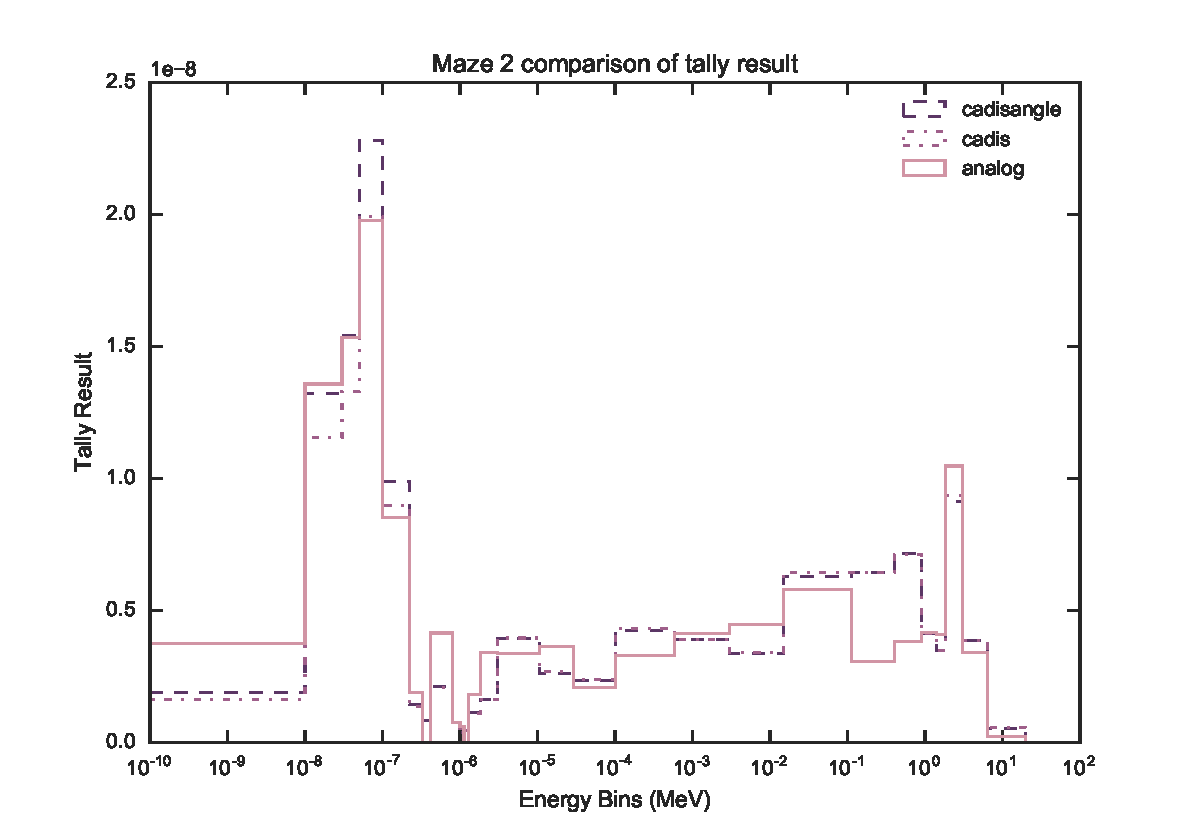
\includegraphics[height=10cm]{./chapters/characterization_probs/figures/char/maze2/maze_2_tally_result_compare.pdf}
  \caption[Tally results comparison between methods for single turn labyrinth.]
  {Tally results comparison between methods for single turn labyrinth.}
  \label{fig:maze2result}
\end{figure}

\begin{figure}[h!]
  \centering
  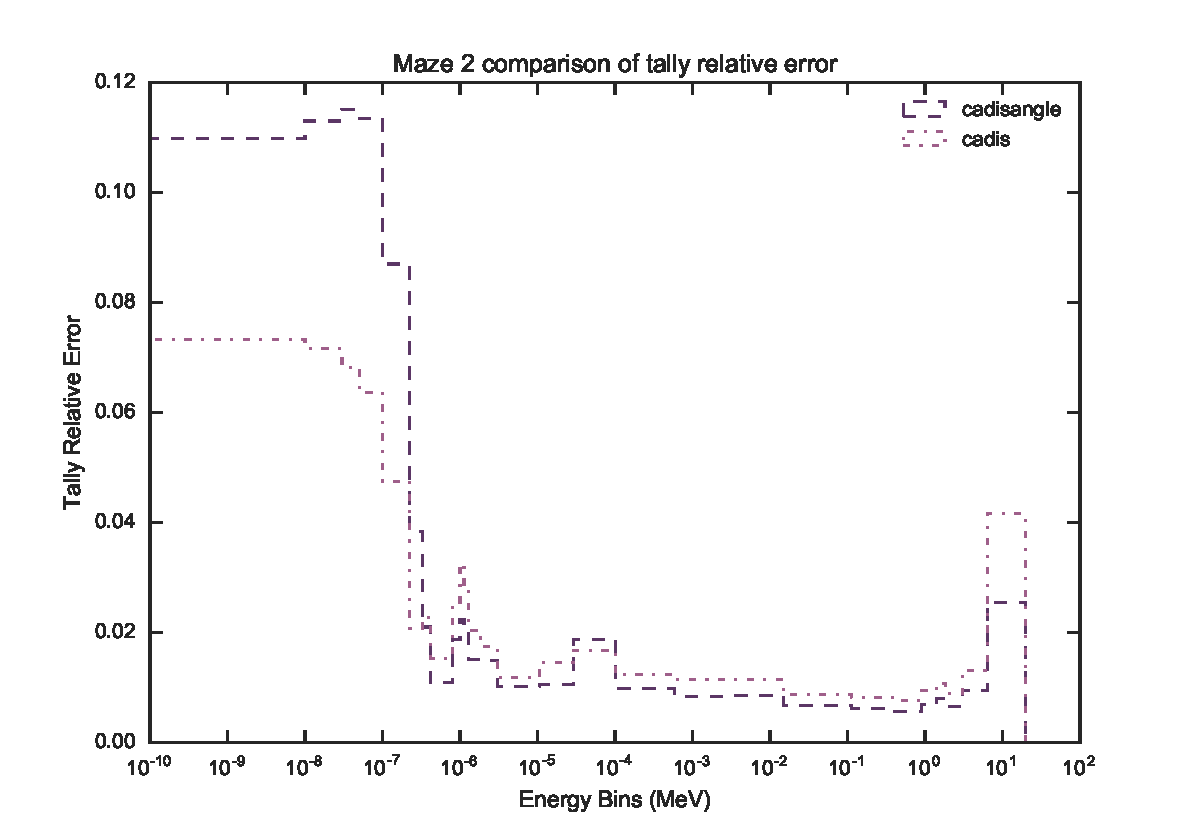
\includegraphics[height=10cm]{./chapters/characterization_probs/figures/char/maze2/maze_2_tally_error_compare.pdf}
  \caption[Tally relative error comparison between methods for single turn
  labyrinth]{Tally relative error comparison between methods for a single turn
  labyrinth.}
  \label{fig:maze2error}
\end{figure}

Figures \ref{fig:maze2result} and \ref{fig:maze2error} show the tally result and
the relative errors for each result in the single turn maze, respectively.
The relative error plot, Figure \ref{fig:maze2error}, does not include the
relative error bins of the analog result because they are significantly higher
than the CADIS and CADIS-$\Omega$ results. This is further confirmed in Table
\ref{tab:maze2foms}, where the minimum relative error FOM is a nontallied bin.
By inspecting Figure \ref{fig:maze2result}, one can observe that the CADIS and
CADIS-$\Omega$ results are in agreement in bins greater that $10^{-7}$ MeV. At
lower energy bins, CADIS-$\Omega$ generally has a higher value for the tally
result than standard CADIS. However, in comparing the errors in these low energy
bins in Figure $\ref{fig:maze2error}$, CADIS has a lower relative error. This
indicates that CADIS sampled many more low-weight particles than CADIS-$\Omega$
in these regions. Conversely, CADIS-$\Omega$ has a lower calculated relative
error than CADIS for bins greater than ~$5*10^{-6}$. This is expected, as
higher energy particles generally exhibit a stronger angular dependence than
low-energy particles. High energy particles exiting the maze towards the tally
detector have much longer mean free paths than the low energy particles, and
will generally show a much stronger effect in the $\Omega$-flux in those
regions. This is illustrated in Figure \ref{fig:}. The shape of the $\Omega$
flux around the detector region is much more strongly dependent on direction in
the high energy group 000 flux than it is for the lower energy group 026 flux.
Despite having lower relative errors than CADIS at higher energies,
CADIS-$\Omega$ has lower FOMs than CADIS for the FOMS calculated with the
minimum relative error. As discussed previously, this is due to the long runtime
of CADIS-$\Omega$, which is more than twice as long as CADIS. From this, we can
conclude that while CADIS-$\Omega$ is better at transporting particles in high
energy regions than CADIS, achieving lower relative errors, the length of time
to do so is prohibitive and achievable by CADIS should the runtimes be the same
for both.

[todo: Omega flux lot of group 00]

[todo: Omega flux plot of group 026]

\subsubsection{Multiple Turn}

The multiple turn labyrinth is built off of the single turn labyrinth geometry.
The labyrinth materials are much the same, but the geometry differs. Table
\ref{tab:maze1foms} summarizes the Figure of Merit results for CADIS,
CADIS-$\Omega$ and nonbiased Monte Carlo. Figures \ref{fig:maze1result} and
\ref{fig:maze1error} show the results obtained by the track length tally in each
method.

\begin{table}[h!]
  \centering
  \begin{tabular}{lrrrrr}
\toprule
{} & cadis &             & cadisangle &             & analog \\
{} &    MC & MC\_adjusted &         MC & MC\_adjusted &     MC \\
\midrule
tally avg   &   327 &         248 &        224 &          71 &  0.054 \\
max RE      &  1.46 &        1.11 &       1.02 &       0.322 & 0.0393 \\
min RE      &   113 &        85.6 &         71 &        22.5 &    -- \\
time (mins) &  51.5 &          68 &       35.5 &         112 &   25.5 \\
\bottomrule
\end{tabular}

  \caption[Figure of Merit comparison for single turn maze.]{Figure of Merit
    comparison for multiple turn maze. The FOMS are
  quantified using three relative error results and two different timing results.
  The relative errors used are the tally average relative error, the tally maximum relative
  error, and the tally minimum relative error; the times are total walltimes for
  the Monte Carlo calculation and the sum of the hybrid method software, the
  deterministic tranport time, and the Monte Carlo calculation time.}
  \label{tab:maze1foms}
\end{table}

\begin{table}[h!]
  \centering
  \begin{tabular}{llrrr}
\toprule
          &              &          cadis &     cadisangle &         analog \\
          &              & time (minutes) & time (minutes) & time (minutes) \\
\midrule
MCNP time & total &          51.52 &          35.55 &          25.46 \\
deterministic time & advantg\_time &           0.25 &           0.21 &            -- \\
          & denovo\_time &          16.28 &          74.85 &            -- \\
          & dispose\_time &           0.01 &           0.40 &            -- \\
          & omega\_time &           0.00 &           1.74 &            -- \\
          & total &          16.53 &          76.80 &            -- \\
wall time &              &          68.05 &         112.35 &          25.46 \\
\bottomrule
\end{tabular}

  \caption[Detailed timing results for multiple turn maze.]
  {Detailed timing results for multiple turn maze.}
  \label{tab:maze1times}
\end{table}

\begin{figure}[h!]
  \centering
  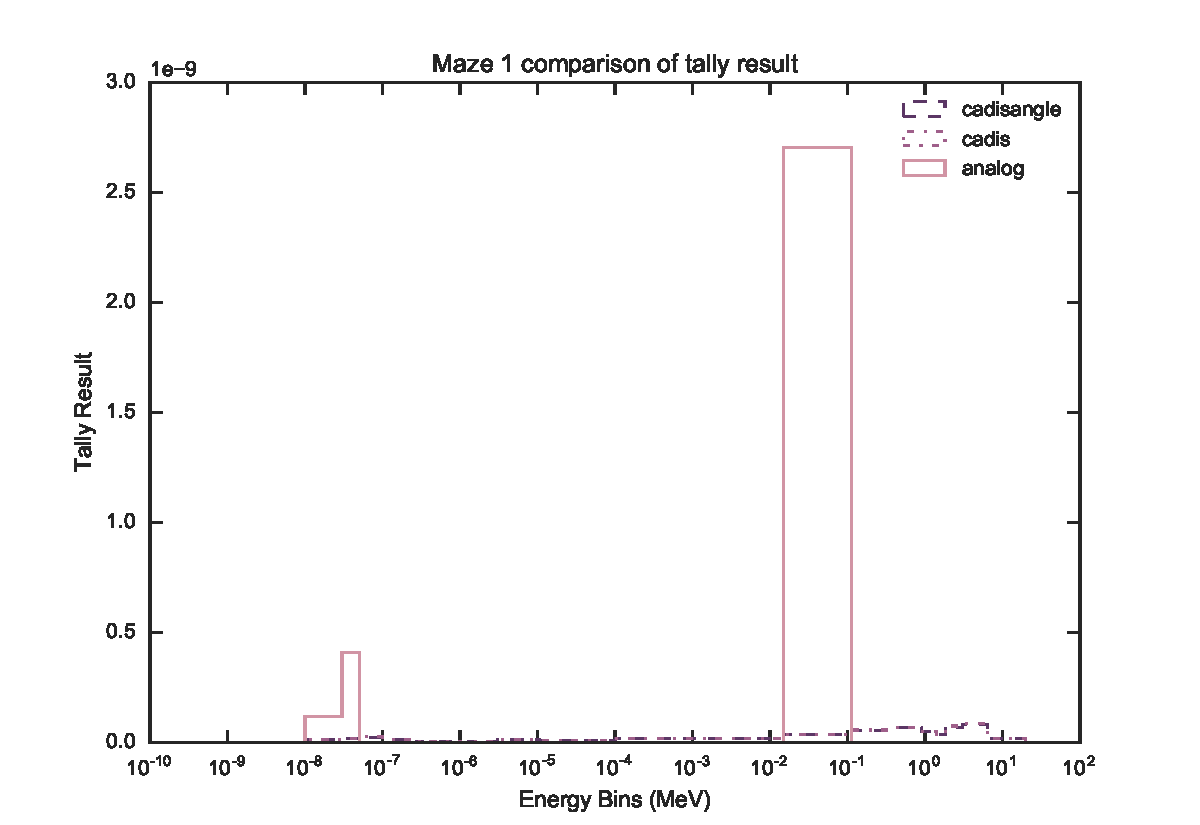
\includegraphics[height=10cm]{./chapters/characterization_probs/figures/char/maze1/maze_1_tally_result_compare.pdf}
  \caption[Tally results comparison between methods for multiple turn labyrinth.]
  {Tally results comparison between methods for multiple turn labyrinth. }
  \label{fig:maze1result}
\end{figure}

\begin{figure}[h!]
  \centering
  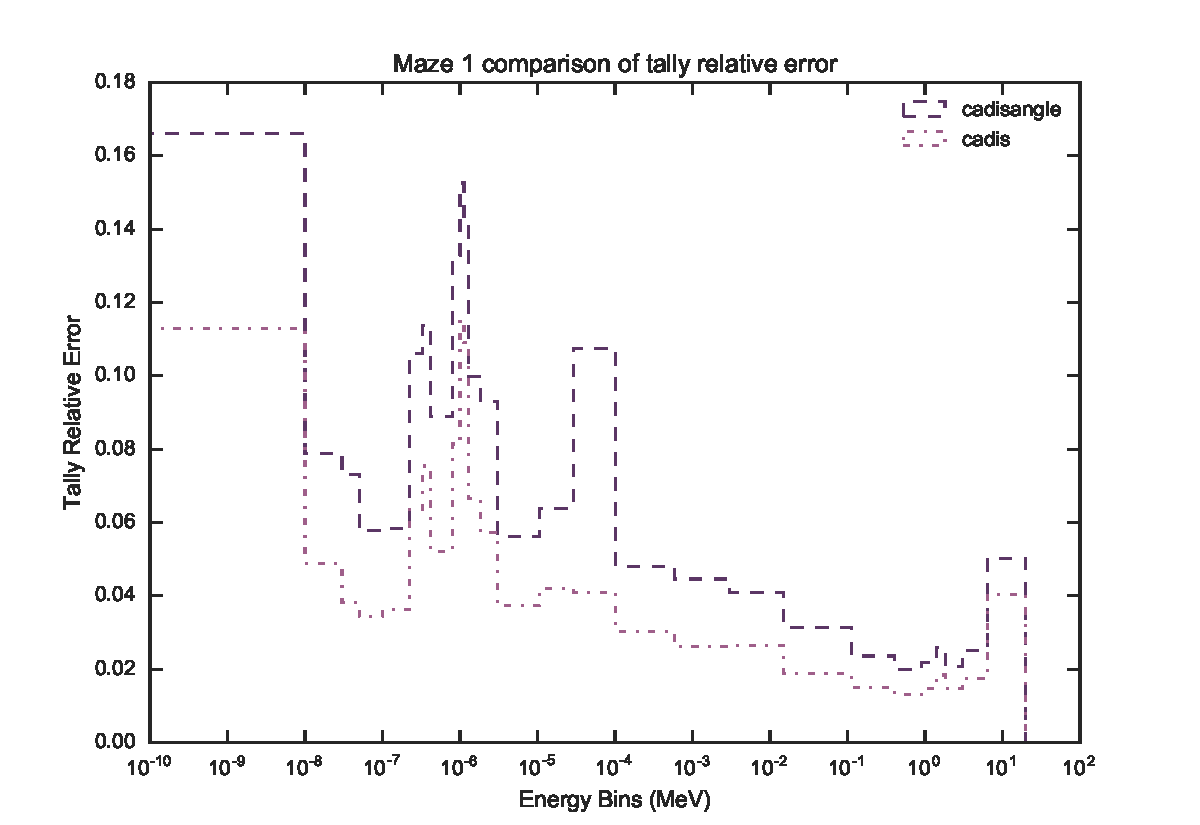
\includegraphics[height=10cm]{./chapters/characterization_probs/figures/char/maze1/maze_1_tally_error_compare.pdf}
  \caption[Tally relative error comparison between methods for multiple turn labyrinth]
  {Tally relative error comparison between methods for a multiple turn
  labyrinth. }
  \label{fig:maze1error}
\end{figure}

% [Summarize results and describe issues affecting performance] \\

\subsection{Steel Beam}
\label{subsec:resultbeam}

\begin{table}[h!]
  \centering
  \begin{tabular}{lrrrrr}
\toprule
{} &    cadis &             & cadisangle &             & analog \\
{} &       MC & MC\_adjusted &         MC & MC\_adjusted &     MC \\
\midrule
tally avg   &      668 &         659 &      3e+03 &    2.96e+03 &   1.39 \\
max RE      &     3.74 &        3.69 &       6.79 &        6.71 & 0.0448 \\
min RE      & 1.43e+03 &    1.41e+03 &   1.33e+03 &    1.31e+03 &    -- \\
time (mins) &      414 &         420 &   2.09e+03 &    2.11e+03 &   22.3 \\
\bottomrule
\end{tabular}

  \caption[Figure of Merit comparison for steel bar embedded in concrete.]
  {Figure of Merit comparison for steel bar embedded in concrete. }
  \label{tab:steelbeamfoms}
\end{table}

\begin{table}[h!]
  \centering
  \begin{tabular}{llrrr}
\toprule
          &             &          CADIS & CADIS-$\Omega$ &         analog \\
        &              & \multicolumn{3}{c}{time (minutes)} \\
\midrule
MCNP time & total &         414.45 &        2086.60 &          22.33 \\
deterministic time & advantg\_time &           0.18 &           0.18 &            -- \\
          & denovo\_time &           5.69 &          25.64 &            -- \\
          & dispose\_time &           0.00 &           0.16 &            -- \\
          & omega\_time &           0.00 &           0.66 &            -- \\
          & total &           5.87 &          26.49 &            -- \\
wall time &              &         420.32 &        2113.09 &          22.33 \\
\bottomrule
\end{tabular}

  \caption[Detailed timing results for steel bar embedded in concrete.]
  {Detailed timing results for steel bar embedded in concrete.}
  \label{tab:steelbeamtimes}
\end{table}

\begin{figure}[h!]
  \centering
  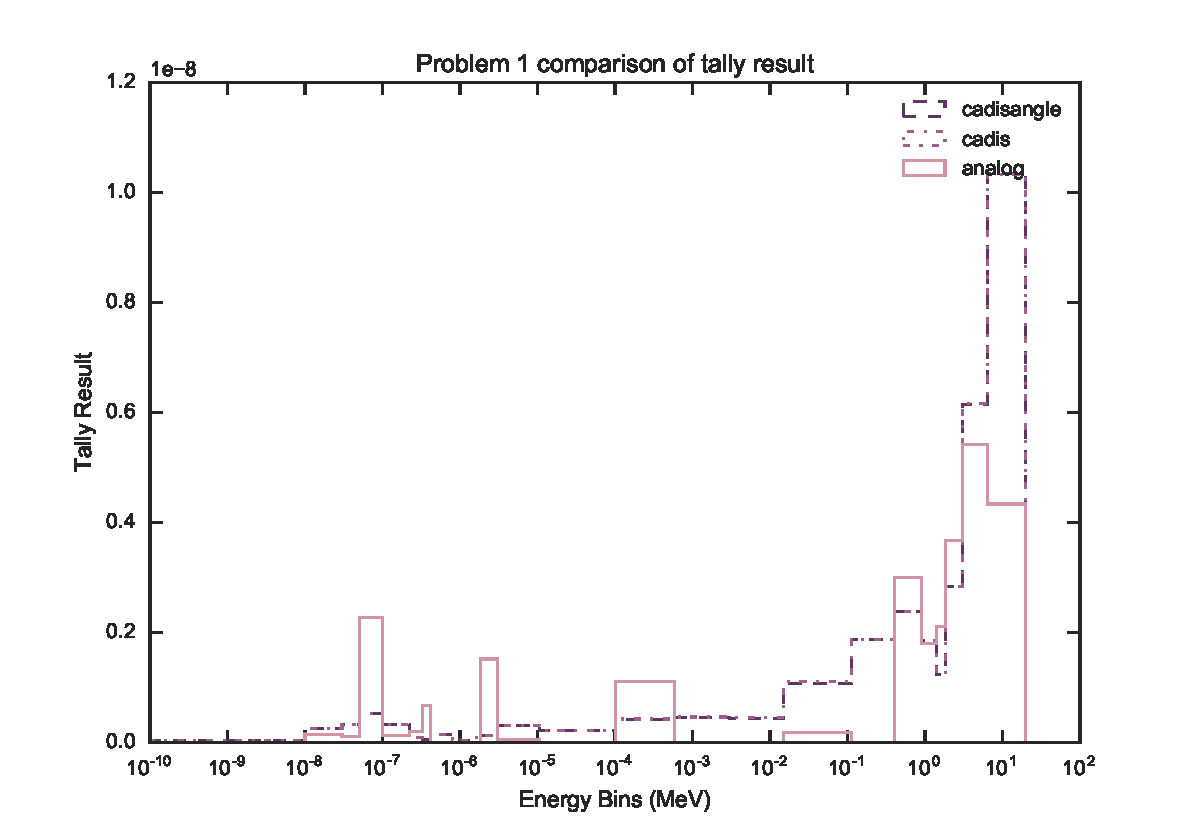
\includegraphics[height=10cm]{./chapters/characterization_probs/figures/char/prob_1/problem_1_tally_result_compare.pdf}
  \caption[Tally results comparison between methods for steel bar embedded in
  concrete.]
  {Tally results comparison between methods for steel bar embedded in concrete.}
  \label{fig:steelbeamresult}
\end{figure}

\begin{figure}[h!]
  \centering
  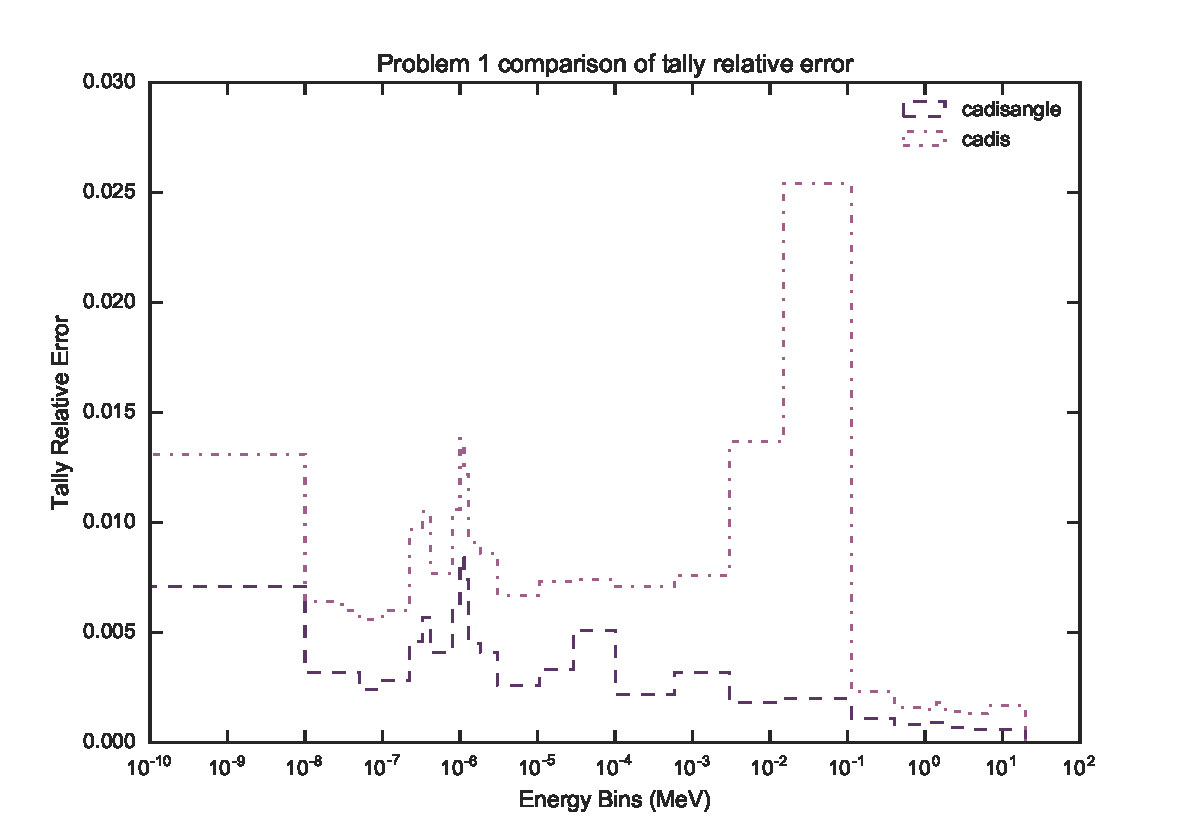
\includegraphics[height=10cm]{./chapters/characterization_probs/figures/char/prob_1/problem_1_tally_error_compare.pdf}
  \caption[Tally relative error comparison between methods for steel bar
  embedded in concrete.]
  {Tally relative error comparison between methods for steel bar embedded in
  concrete.}
  \label{fig:steelbeamerror}
\end{figure}
% [Table of FOMs for this problem] \\
%
% [Plot of tally results for this problem] \\
%
% [Plot of anisotropies for this problem] \\
%
% [Summarize results and describe issues affecting performance] \\

\subsection{U-Shaped Corridor}
\label{subsec:resultsucorridor}

\begin{table}[h!]
  \centering
  \begin{tabular}{lrrrrr}
\toprule
{} &  cadis &             & cadisangle &             & analog \\
{} &     MC & MC\_adjusted &         MC & MC\_adjusted &     MC \\
\midrule
tally avg   &   64.1 &        51.9 &       60.2 &        38.3 &  0.378 \\
max RE      & 0.0183 &      0.0148 &     0.0144 &     0.00913 & 0.0644 \\
min RE      &   14.9 &          12 &       13.4 &        8.54 &    -- \\
time (mins) &   54.6 &        67.5 &        188 &         296 &   15.5 \\
\bottomrule
\end{tabular}

  \caption[Figure of Merit comparison between methods for U-shaped air corridor in concrete.]
  {Figure of Merit comparison between methods for U-shaped air corridor in
  concrete.}
  \label{tab:ucorridorfoms}
\end{table}

\begin{table}[h!]
  \centering
  \begin{tabular}{llrrr}
\toprule
          &             &          CADIS & CADIS-$\Omega$ &         analog \\
        &              & \multicolumn{3}{c}{time (minutes)} \\
\midrule
MCNP time & total &          54.61 &         187.92 &          15.54 \\
deterministic time & advantg\_time &           0.19 &           0.21 &            -- \\
          & denovo\_time &          12.68 &         105.90 &            -- \\
          & dispose\_time &           0.01 &           0.35 &            -- \\
          & omega\_time &           0.00 &           1.49 &            -- \\
          & total &          12.87 &         107.60 &            -- \\
wall time &              &          67.48 &         295.52 &          15.54 \\
\bottomrule
\end{tabular}

  \caption[Detailed timing results for U-shaped air corridor in concrete.]
  {Detailed timing results for U-shaped air corridor in concrete.}
  \label{tab:ucorridortimes}
\end{table}

\begin{figure}[h!]
  \centering
  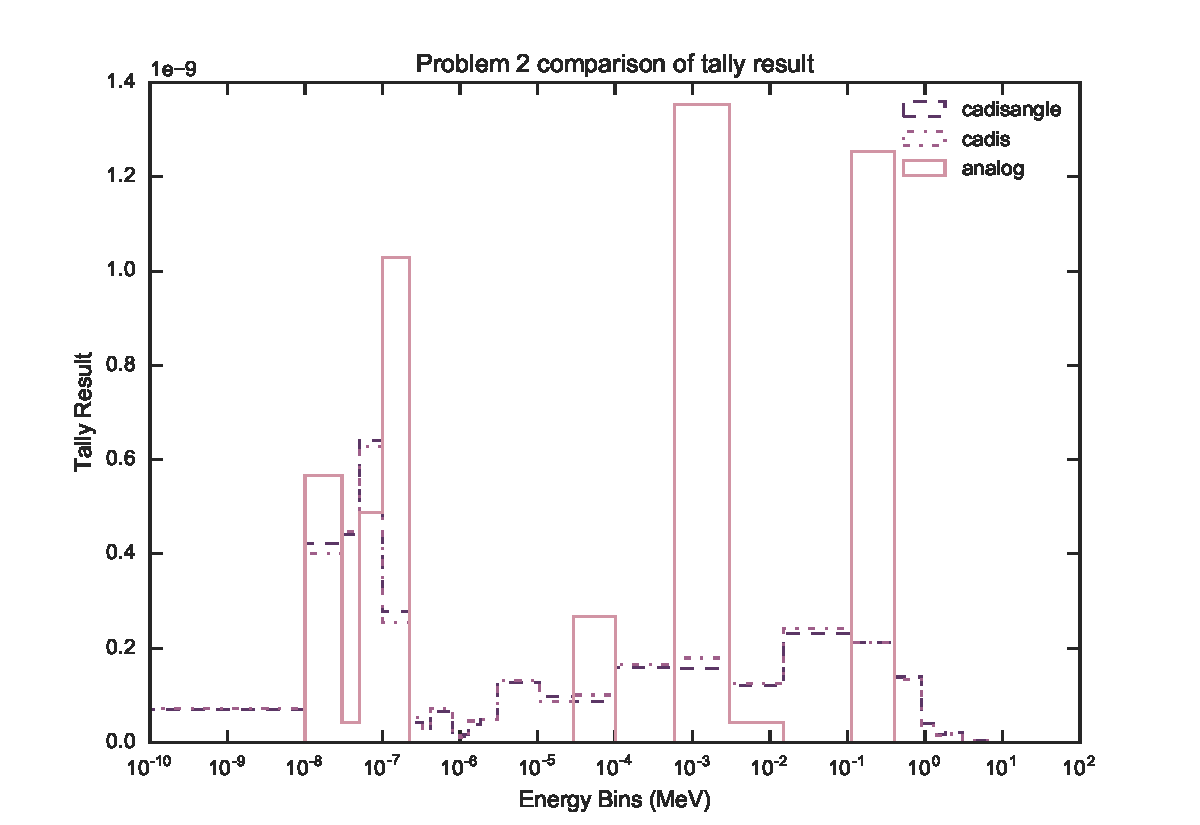
\includegraphics[height=10cm]{./chapters/characterization_probs/figures/char/prob_2/problem_2_tally_result_compare.pdf}
  \caption[Tally results comparison between methods for U-shaped air corridor in
  concrete.]
  {Tally results comparison between methods for U-shaped air corridor in
  concrete.}
  \label{fig:ucorridorresult}
\end{figure}

\begin{figure}[h!]
  \centering
  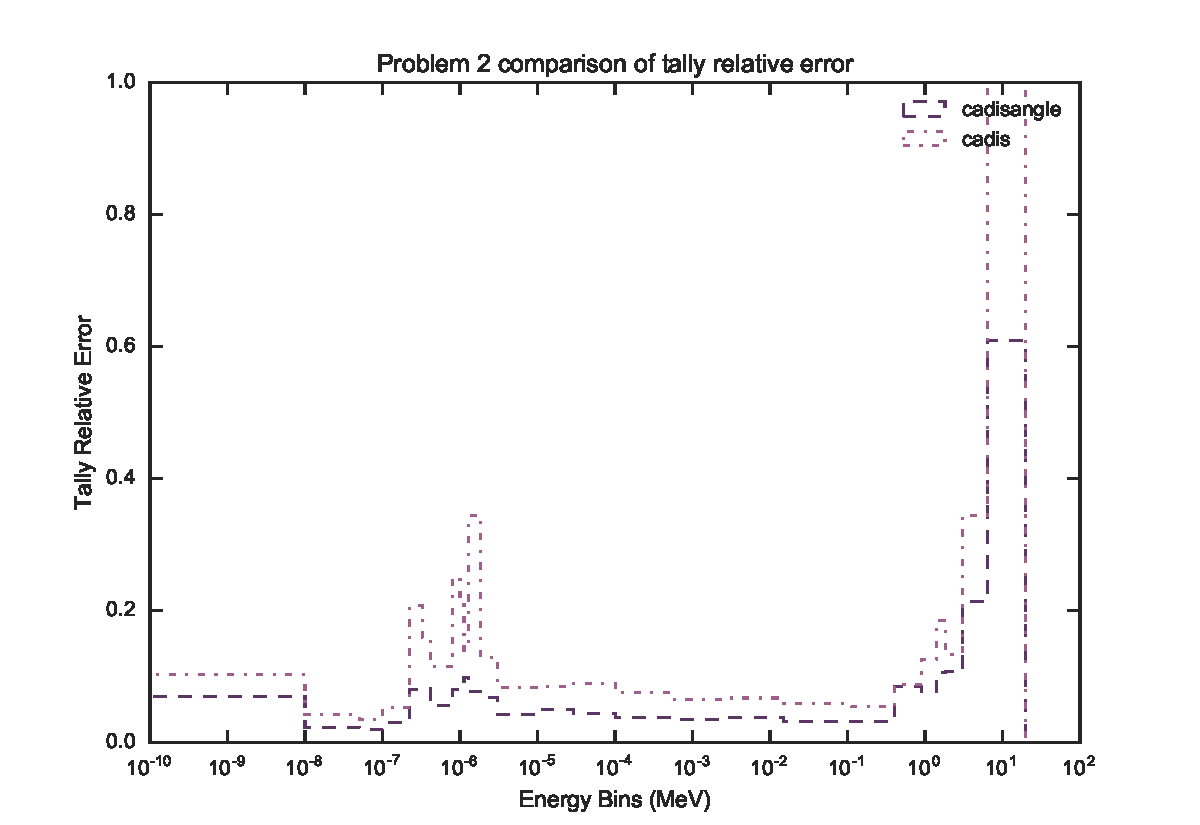
\includegraphics[height=10cm]{./chapters/characterization_probs/figures/char/prob_2/problem_2_tally_error_compare.pdf}
  \caption[Tally relative error comparison between methods for U-shaped air
  corridor in concrete.]
  {Tally relative error comparison between methods for U-shaped air corridor in
  concrete.}
  \label{fig:ucorridorerror}
\end{figure}
% [Table of FOMs for this problem] \\
%
% [Plot of tally results for this problem] \\
%
% [Plot of anisotropies for this problem] \\
%
% [Summarize results and describe issues affecting performance] \\

\subsection{Shielding with Rebar}
\label{subsec:resultrebar}

\begin{table}[h!]
  \centering
  \begin{tabular}{lrrrrr}
\toprule
{} & \multicolumn{2}{c}{CADIS}   & \multicolumn{2}{c}{CADIS-$\Omega$}  & analog \\
{} &    MC & MC$_{hybrid}$ &         MC & MC$_{hybrid}$ &     MC \\
\midrule
tally avg   &   1.15 &        1.09 &     0.0136 &      0.0127 &  0.948 \\
max RE      & 0.0345 &      0.0327 &    0.00117 &     0.00109 & 0.0186 \\
min RE      &    235 &         223 &        199 &         186 &    -- \\
time (mins) &    328 &         346 &   1.55e+03 &    1.66e+03 &   53.8 \\
\bottomrule
\end{tabular}

  \caption[Figure of Merit comparison between methods for rebar-embedded
  concrete.]{Figure of Merit comparison between methods for rebar-embedded
  concrete.}
  \label{tab:rebarfoms}
\end{table}

\begin{table}[h!]
  \centering
  \begin{tabular}{llrrr}
\toprule
          &              &          cadis &     cadisangle &         analog \\
          &              & time (minutes) & time (minutes) & time (minutes) \\
\midrule
MCNP time & total &         327.81 &        1550.54 &          53.82 \\
deterministic time & advantg\_time &           0.28 &           0.29 &            -- \\
          & denovo\_time &          17.70 &         105.09 &            -- \\
          & dispose\_time &           0.03 &           0.41 &            -- \\
          & omega\_time &           0.00 &           2.05 &            -- \\
          & total &          17.98 &         107.43 &            -- \\
wall time &              &         345.79 &        1657.97 &          53.82 \\
\bottomrule
\end{tabular}

  \caption[Detailed timing results for rebar-embedded concrete]
  {Detailed timing results for rebar-embedded concrete.}
  \label{tab:rebartimes}
\end{table}

\begin{figure}[h!]
  \centering
  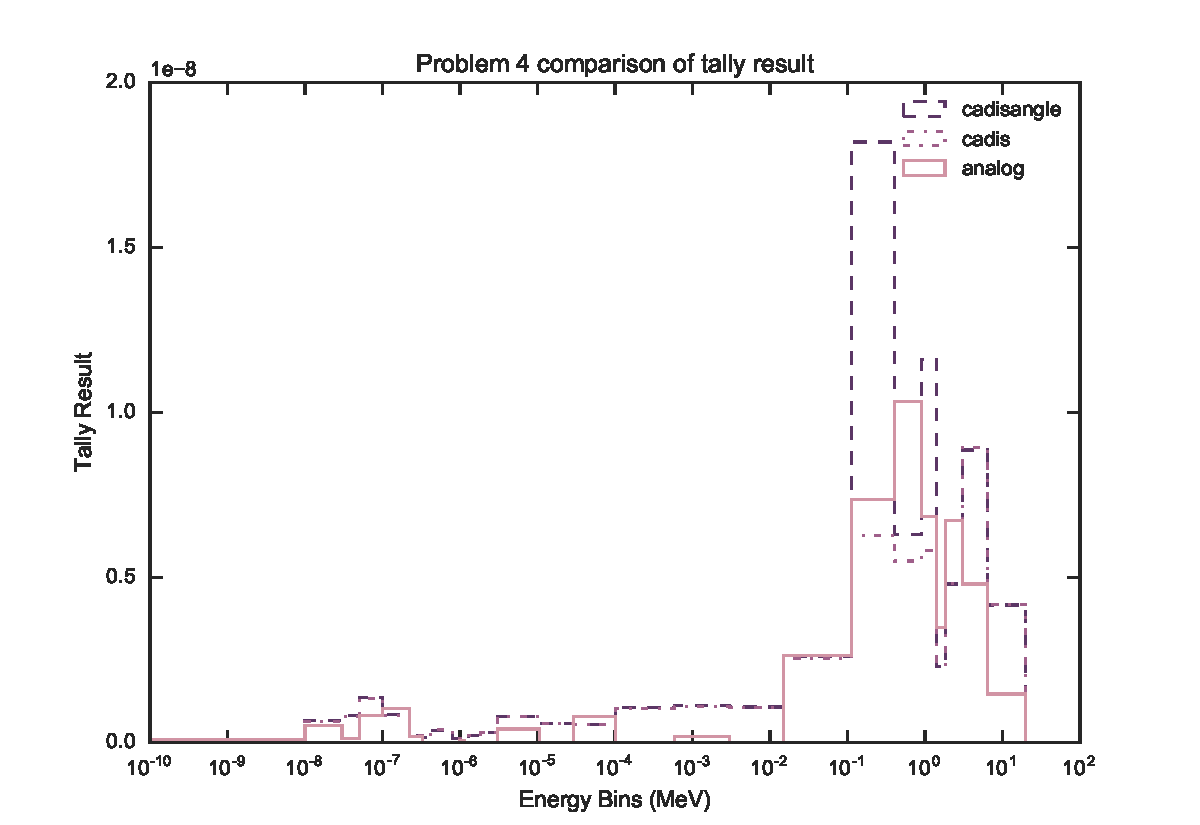
\includegraphics[height=10cm]{./chapters/characterization_probs/figures/char/prob_4/problem_4_tally_result_compare.pdf}
  \caption[Tally results comparison between methods for rebar-embedded concrete.]
  {Tally results comparison between methods for rebar-embedded concrete.}
  \label{fig:rebarresult}
\end{figure}

\begin{figure}[h!]
  \centering
  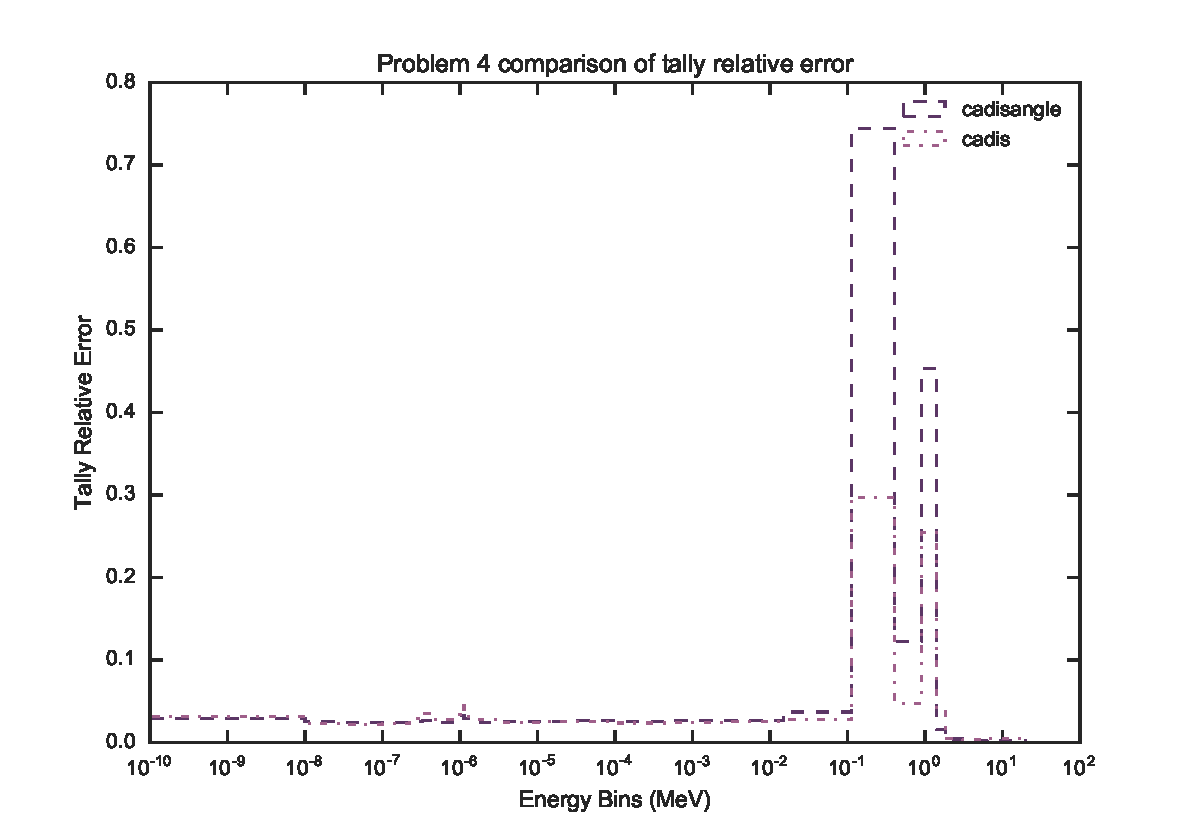
\includegraphics[height=10cm]{./chapters/characterization_probs/figures/char/prob_4/problem_4_tally_error_compare.pdf}
  \caption[Tally relative error comparison between methods for rebar-embedded concrete.]
  {Tally relative error comparison between methods for rebar-embedded concrete.}
  \label{fig:rebarerror}
\end{figure}
% [Table of FOMs for this problem] \\
%
% [Plot of tally results for this problem] \\
%
% [Plot of anisotropies for this problem] \\
%
% [Summarize results and describe issues affecting performance] \\

\subsection{Beam Problem}
\label{subsec:resultsbeam}

\begin{table}[h!]
  \centering
  \begin{tabular}{lrrrrr}
\toprule
{} & cadis &             & cadisangle &             & analog \\
{} &    MC & MC\_adjusted &         MC & MC\_adjusted &     MC \\
\midrule
tally avg   &   368 &         138 &       94.8 &        7.91 &    317 \\
max RE      & 0.542 &       0.202 &       1.18 &      0.0984 &    1.6 \\
min RE      &   -- &         -- &        -- &         -- &    -- \\
time (mins) &  2.23 &        5.97 &       1.69 &        20.3 &   1.69 \\
\bottomrule
\end{tabular}

  \caption[Figure of Merit comparison between methods for simplified
    experimental nuclear physics beamline.]
    {Figure of Merit comparison between methods for simplified experimental
    nuclear physics beamline.}
  \label{tab:beamfoms}
\end{table}

\begin{table}[h!]
  \centering
  \begin{tabular}{llrrr}
\toprule
          &             &          CADIS & CADIS-$\Omega$ &         analog \\
        &              & \multicolumn{3}{c}{time (minutes)} \\
\midrule
MCNP time & total &           2.23 &           1.69 &           1.69 \\
deterministic time & advantg\_time &           0.17 &           0.15 &            -- \\
          & denovo\_time &           3.57 &          17.88 &            -- \\
          & dispose\_time &           0.00 &           0.12 &            -- \\
          & omega\_time &           0.00 &           0.53 &            -- \\
          & total &           3.74 &          18.56 &            -- \\
wall time &              &           5.97 &          20.25 &           1.69 \\
\bottomrule
\end{tabular}

  \caption[Detailed timing results for simplified experimental nuclear physics
  beamline.]
  {Detailed timing results for simplified experimental nuclear physics beamline.}
  \label{tab:steelbeamtimes}
\end{table}

\begin{figure}[h!]
  \centering
  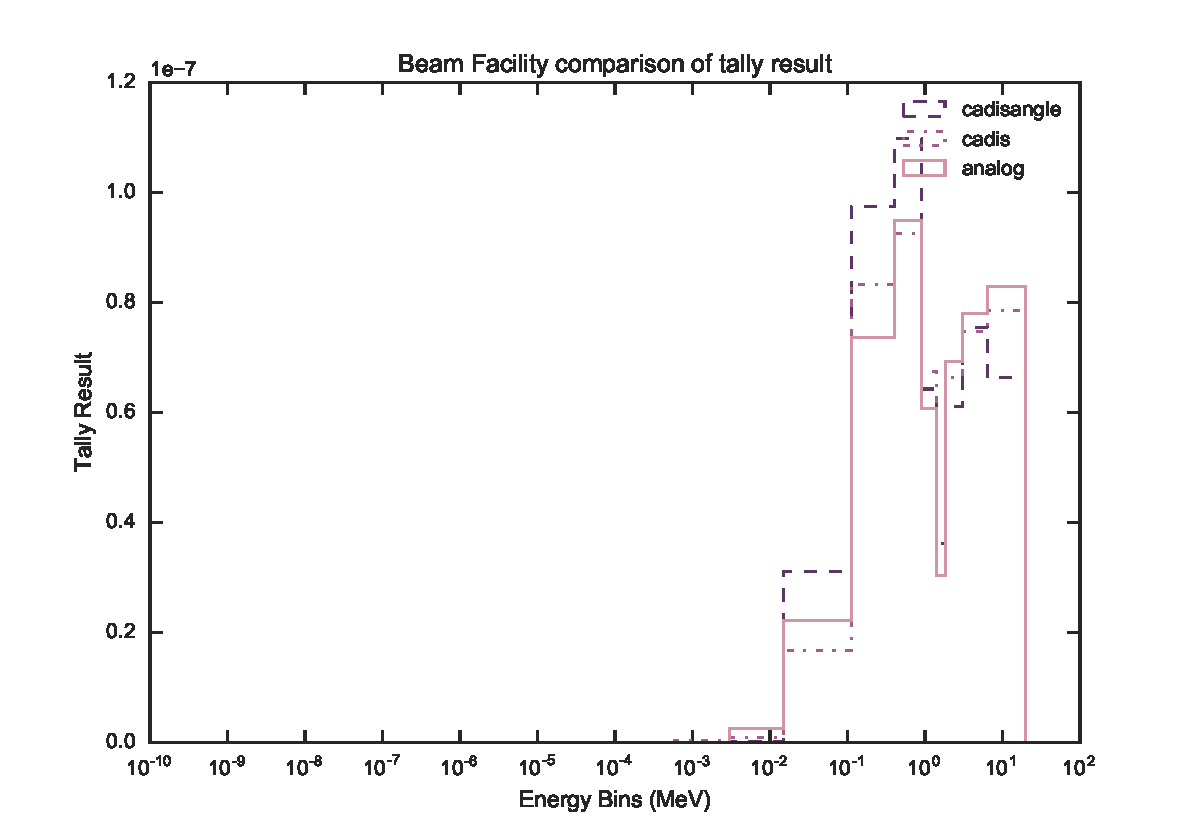
\includegraphics[height=10cm]{./chapters/characterization_probs/figures/char/beam/beam_facility_tally_result_compare.pdf}
  \caption[Tally results comparison between methods for simplified experimental
    nuclear physics beamline.]
  {Tally results comparison between methods for simplified experimental
    nuclear physics beamline.}
  \label{fig:beamresult}
\end{figure}

\begin{figure}[h!]
  \centering
  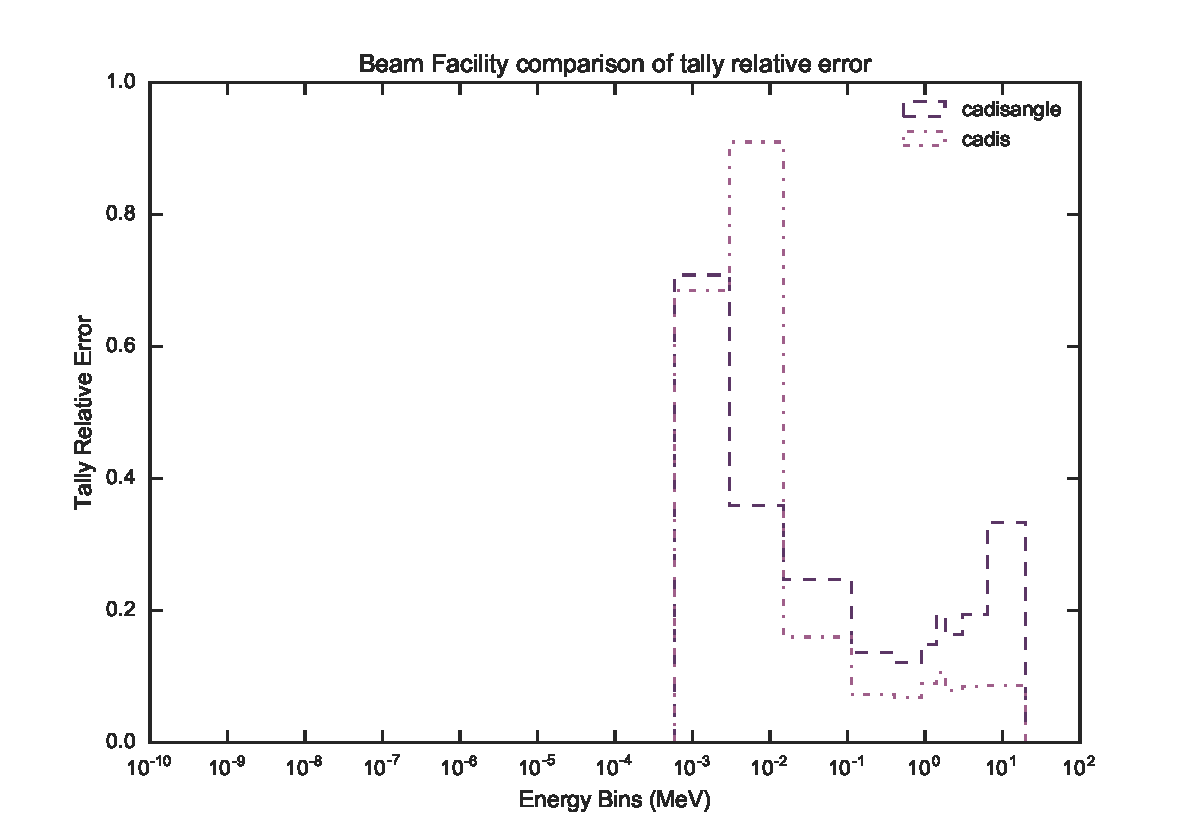
\includegraphics[height=10cm]{./chapters/characterization_probs/figures/char/beam/beam_facility_tally_error_compare.pdf}
  \caption[Tally relative error comparison between methods
    for simplified experimental nuclear physics beamline.]
  {Tally relative error comparison between methods for simplified experimental
    nuclear physics beamline.}
  \label{fig:beamerror}
\end{figure}
% [Table of FOMs for this problem] \\
%
% [Plot of tally results for this problem] \\
%
% [Plot of anisotropies for this problem] \\
%
% [Summarize results and describe issues affecting performance] \\

\subsection{Therapy Room}
% \label{subsec:resultstherapy}
% \begin{table}[h!]
%   \centering
%   \input{./chapters/characterization_probs/figures//_tally_foms_compare}
%   \caption[]{}
%   \label{tab:foms}
% \end{table}

% \begin{figure}[h!]
%   \centering
%   \includegraphics[height=10cm]{./chapters/characterization_probs/figures/char/_tally_result_compare.pdf}
%   \caption[Tally results comparison between methods for ]
%   {Tally results comparison between methods for }
%   \label{fig:result}
% \end{figure}

% \begin{figure}[h!]
%   \centering
%   \includegraphics[height=10cm]{./chapters/characterization_probs/figures/char/_tally_error_compare.pdf}
%   \caption[Tally relative error comparison between methods for ]
%   {Tally relative error comparison between methods for}
%   \label{fig:result}
% \end{figure}
% [Table of FOMs for this problem] \\
%
% [Plot of tally results for this problem] \\
%
% [Plot of anisotropies for this problem] \\
%
% [Summarize results and describe issues affecting performance] \\

